\documentclass{beamer}
\usepackage{listings}

\usetheme{DarkConsole}
%Information to be included in the title page:
\title{Raylib: Graphics Library for C/C++}
\author{Rick C. de Baca}
\date{03.26.26}

\titlegraphic{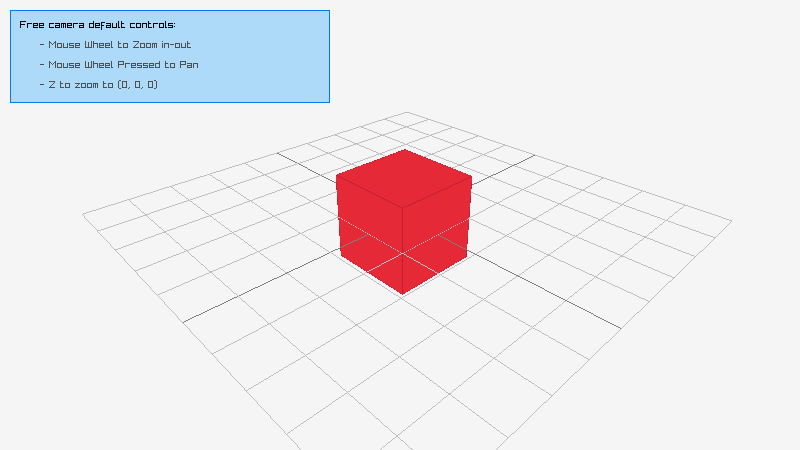
\includegraphics[width=90mm]{images/raylib_title.png}}

% \renewcommand*{\familydefault}{\rmdefault}

\definecolor{codegreen}{rgb}{0.22, 1.0, 0.08}
\definecolor{codegray}{rgb}{0.5,0.5,0.5}
\definecolor{codepurple}{rgb}{0.58,0,0.82}
\definecolor{backcolour}{rgb}{0.95,0.95,0.92}
\definecolor{darkgray}{rgb}{0.3,0.3,0.3}

\lstnewenvironment{simula}
{
 \lstset{
 	language=C++, % choose the language of the code.
 	frame=single,
 	tabsize=2,
 	rulesepcolor=\color{white},
 	rulecolor=\color{white},
  backgroundcolor=\color{darkgray},   
  commentstyle=\color{white},
  keywordstyle=\color{white},
  numberstyle=\tiny\color{white},
  stringstyle=\color{white},
  basicstyle=\tiny\ttfamily,
  breakatwhitespace=false,         
  breaklines=true,                 
  captionpos=b,                    
  keepspaces=true,                 
  numbers=left,                    
  numbersep=5pt,                  
  showspaces=false,                
  showstringspaces=false,
  showtabs=false,                  
  tabsize=2
}
}
{}

\begin{document}

\frame{\titlepage}

\begin{frame}[fragile]
\frametitle{Raylib}

\begin{itemize}
  
\item raylib is a simple and easy-to-use graphics library.

\item raylib is highly inspired by Borland BGI graphics lib and by XNA
framework and it's especially well suited for prototyping, tooling,
graphical applications, embedded systems and education.

\item https://github.com/raysan5/raylib
\item https://www.raylib.com/

\end{itemize}

\end{frame}

\begin{frame}[fragile]
  \frametitle{raylib features}

  \begin{itemize}
  \item NO external dependencies, all required libraries included with raylib
  \item Multiplatform: Windows, Linux, MacOS, RPI, Android, ...
  \item Hardware accelerated with OpenGL (1.1, 2.1, 3.3, 4.3 or ES 2.0)
  \item Powerful Fonts module (SpriteFonts, BMfonts, TTF, SDF)
  \item Multiple texture formats support, including compressed formats (DXT, ETC, ASTC)
  \item Animated 3d models supported (skeletal bones animation)
  \item Audio loading and playing with streaming support (WAV, OGG, MP3, FLAC, XM, MOD)
  \item Huge examples collection with +120 code examples.
  \item Bindings to +60 programming languages.
  \item Free and open source.
    \end{itemize}

\end{frame}

\begin{frame}[fragile]
\frametitle{Video Game Example (home)}
  
  \begin{figure}[ht!]
    \centering
    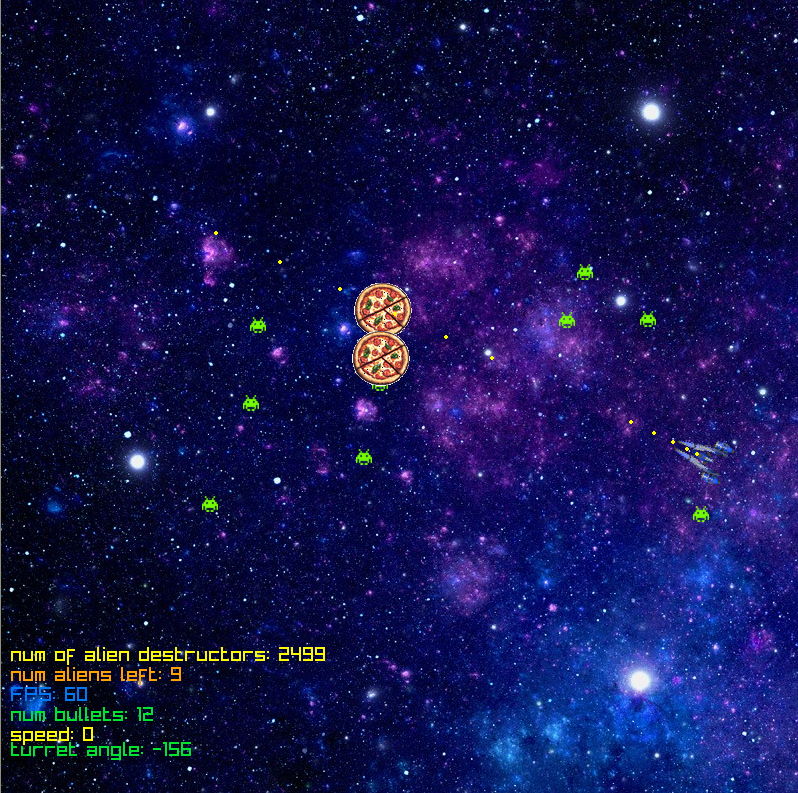
\includegraphics[width=80mm]{images/ship_pizza.png}
    \label{overflow}
  \end{figure}
  
\end{frame}

\begin{frame}[fragile]
  \frametitle{Work Example}

  \begin{figure}[ht!]
    \centering
    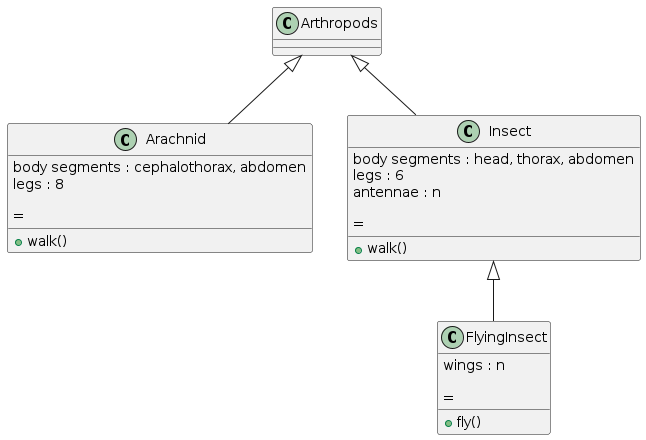
\includegraphics[width=100mm]{images/bugs.png}
    \label{overflow}
  \end{figure}
  
\end{frame}

\begin{frame}[fragile]
\frametitle{Code Example}

  \begin{simula}

  // Main game loop
	while (!WindowShouldClose())    // Detect window close button or ESC key
    {
				BeginDrawing();
	  		ClearBackground(RAYWHITE);
			
  			if (!paused) {
	  			theGrid.draw();
		  	}
			
			 // Print FPS
			 std::stringstream fps_msg;
			 fps_msg << "FPS: " << GetFPS();
			
			 DrawText(fps_msg.str().c_str(), 10, 700, 20, BLUE);
			
			EndDrawing();
    }
	
	CloseWindow();        // Close window and OpenGL context
	    
  \end{simula}
  
\end{frame}


\begin{frame}[fragile]
\frametitle{Code Example (2)}

  \begin{simula}

    using SpriteVector = std::vector<std::unique_ptr<Sprite>>;
    using ExplosionVector = std::vector<std::unique_ptr<Particles>>;
  
    // Start loading assets and creating sprites.
	
	  Sound fire_bullet = LoadSound( std::string(asset_dir + "sounds/heat-vision.mp3").c_str() );

    // Load Background
    
    Texture2D background = LoadTexture( std::string(asset_dir + "backgrounds/blue_nebula.png").c_str());
    
    // Create Player
    
    Entity ship("./assets/sprites/blue_ship_64.png", 50, 50, 47, 64);
    ship.sprite_->accel_ = -0.01;
	  
	  SpriteVector aliens;
    aliens.push_back(std::make_unique<Sprite>(sprite_path,
	                   GameMath::RandInt(screen_width),
		                 GameMath::RandInt(screen_height),
			               size, size) );
  }
	    
  \end{simula}
  
\end{frame}

\end{document}

